\documentclass[12pt]{article}
\usepackage{graphicx}
\usepackage{subcaption}
\usepackage{setspace}

\usepackage{amsmath,amsfonts,amssymb,amscd}
\pagestyle{myheadings}
\markright{\underline{\today ~~~~~~~~~~~~~~  HPC21 ~~~~~~~~~~~~~  Jeff McFadden}}

\setlength{\textwidth}{6.25in}
\setlength{\textheight}{8.5in}
\setlength{\oddsidemargin}{0.0in}
\setlength{\topmargin}{0.0in}

\renewcommand{\baselinestretch}{1.5}

\newcommand{\lj}{\mbox{$[\kern-0.1478125em[$}}
\newcommand{\rj}{\mbox{$]\kern-0.1478125em]$}}
\newcommand{\bbS}{\mathbb{S}}
\newcommand{\bbT}{\mathbb{T}}
\newcommand{\bbI}{\mathbb{I}}
\newcommand{\BFX}{{\bf x}}
\newcommand{\BFB}{{\bf B}}
\newcommand{\BFJ}{{\bf J}}
\newcommand{\BFK}{{\bf K}}
\newcommand{\BFI}{{\bf I}}
\newcommand{\BFT}{{\bf t}}
\newcommand{\BFS}{{\bf S}}
\newcommand{\BFII}{{\bf II}}
\newcommand{\BFe}{{\bf e}}
\newcommand{\BFw}{{\bf w}}
\newcommand{\BFA}{{\bf A}}
\newcommand{\BFrh}{\widehat{r}}
\newcommand{\BFth}{\widehat{\theta}}
\newcommand{\BFph}{\widehat{\phi}}
\newcommand{\BFC}{{\bf \chi}}
\newcommand{\be}{\begin{equation}}
\newcommand{\ee}{\end{equation}}
\newcommand{\BFn}{{\bf n}}
\newcommand{\BFx}{\widehat{{\bf x}}}
\newcommand{\BFxi}{\widehat{{\bf \xi}}}
\newcommand{\BFy}{\widehat{{\bf y}}}
\newcommand{\BFz}{\widehat{{\bf z}}}
\newcommand{\BFr}{\widehat{{\bf r}}}
\newcommand{\BFt}{\widehat{{\boldmath \theta}}}

\begin{document}

\section*{Ex.~2.2}

These results are for a CIMS linux box with the 'lscpu' output:
\begin{singlespace}
\begin{verbatim}
box$ lscpu
Architecture:          x86_64
CPU(s):                8
On-line CPU(s) list:   0-7
Model name:            Intel(R) Core(TM) i7-4770 CPU @ 3.40GHz
CPU MHz:               3400.000
L1d cache:             32K
L1i cache:             32K
L2 cache:              256K
L3 cache:              8192K
\end{verbatim}
\end{singlespace}

\noindent We compile with the flags 
\begin{verbatim}
   CFLAGS = -std=c++11 -g -O3 -march=native
\end{verbatim}

\subsection*{Unblocked Results}

We refer to the example \rm{MMult1.cpp} with the function:
\begin{singlespace}
\begin{verbatim}
void MMult1(long m, long n, long k, double *a, double *b, double *c) {
  for (long j = 0; j < n; j++) {
    for (long p = 0; p < k; p++) {
      for (long i = 0; i < m; i++) {
        double A_ip = a[i+p*m];
        double B_pj = b[p+j*k];
        double C_ij = c[i+j*m];
        C_ij = C_ij + A_ip * B_pj;
        c[i+j*m] = C_ij;
\end{verbatim}
\end{singlespace}
\noindent as 'jpi' (indicating the order of the 'for' loops).
If we consider the six permutations of the order of the loops,
we see the results in Fig.~1. The 'jpi' ordering has the highest
flop rate,\footnote{We
note that this is the same ordering
that is used in the reference version (unblocked) of the BLAS routine
'dgemm'\cite{dgemm}.} followed by 'pji'. For 'jpi' the index 'i' is the inner-most
loop, corresponding to data access along 
the columns of $C(i,j)$ and $A(i,p)$.
The effect of cache size on the flop rate
is apparent for $N \approx 150$ and $N \approx 1000$.

\begin{figure}[ht]
\vspace*{-0.05in}
\centering
    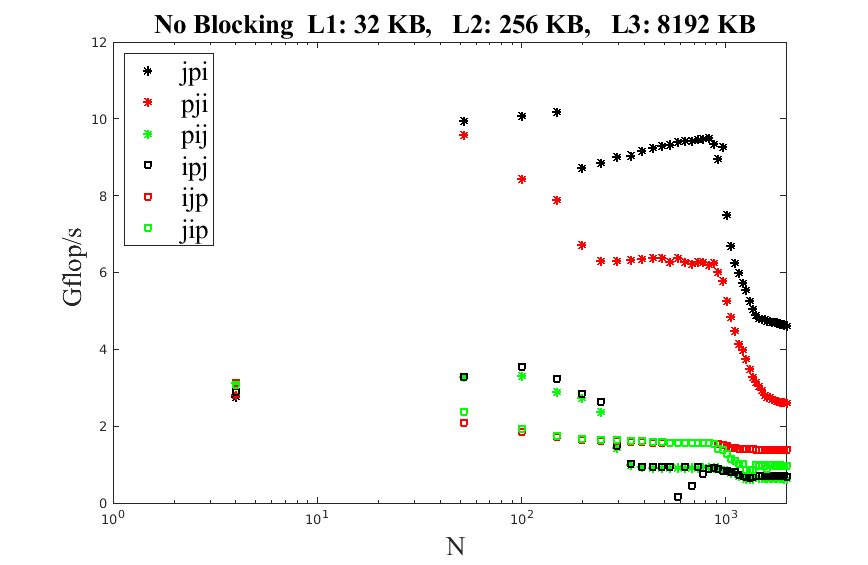
\includegraphics[width=0.8\textwidth]{Fig_1.png}
  \caption{Flop rate versus matrix dimension N for various
           loop orderings, denoted by, e.g., 'jpi' as in the text.}
  \label{fig1}
\end{figure}

\subsection*{Blocking}

From henceforth we consider only the 'jpi' ordering.

\subsubsection*{Block the Inner Loop}

We first block the inner loop ('i'):
\begin{singlespace}
\begin{verbatim}
  for (long j = 0; j < n; j++) {
    for (long p = 0; p < k; ++p) {
      double B_pj = b[p+j*k];
      for (long ib = 0; ib < m; ib+=BLOCK_SIZE) {

        for (long i = ib; i < ib+BLOCK_SIZE; ++i) {
          double A_ip = a[i+p*m];
          double C_ij = c[i+j*m];
          C_ij = C_ij + A_ip * B_pj;
          c[i+j*m] = C_ij;
\end{verbatim}
\end{singlespace}

Results are shown in Figure~2. The best flop rate of about 17.7 Gflops/s
for $N \approx 50$ is for a BLOCKSIZE of 8, which is better than the unblocked
case (rate of about 10 Gflops/s). 
Rates for $N > 150$ are only slightly better than the unblocked case,
and for $Ni > 1000$ the results all asymptote.

\begin{figure}[ht]
\vspace*{-0.05in}
\centering
    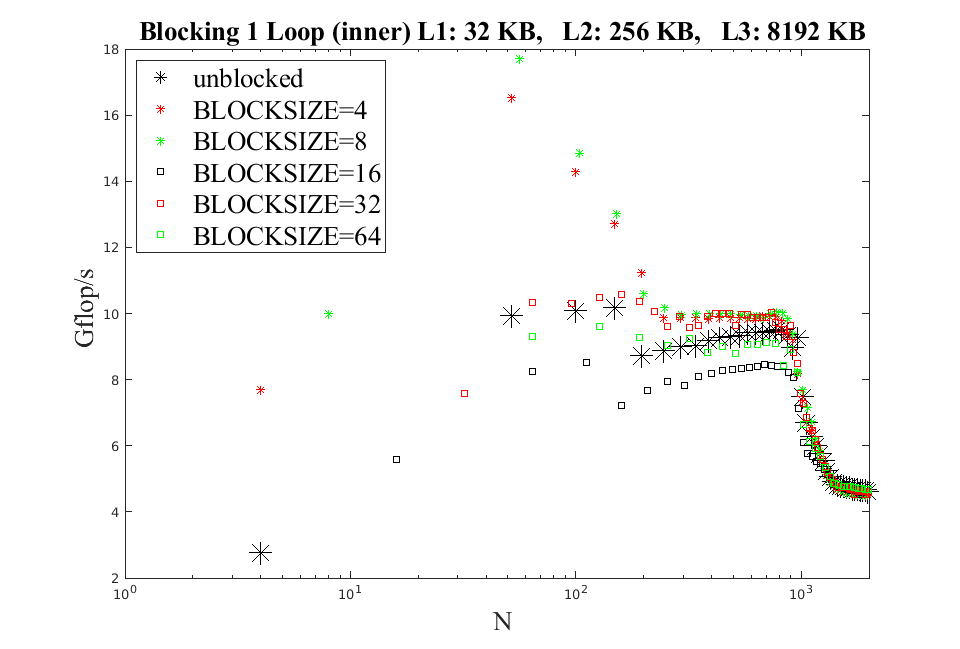
\includegraphics[width=0.8\textwidth]{Fig_2.png}
  \caption{Flop rate versus matrix dimension N for the 'jpi'
           loop ordering and blocking of the two inner-most loops,
           for various values of BLOCK\_SIZE.}
  \label{fig2}
\end{figure}

\subsubsection*{Block the Two Inner-Most Loops}

We next block the two innermost loops:
\begin{singlespace}
\begin{verbatim}
  for (long j = 0; j < n; j++) {

    for (long pb = 0; pb < k; pb+=BLOCK_SIZE) {
      for (long ib = 0; ib < m; ib+=BLOCK_SIZE) {

        for (long p = pb; p < pb+BLOCK_SIZE; ++p) {
          double B_pj = b[p+j*k];
          for (long i = ib; i < ib+BLOCK_SIZE; ++i) {
            double A_ip = a[i+p*m];
            double C_ij = c[i+j*m];
            C_ij = C_ij + A_ip * B_pj;
            c[i+j*m] = C_ij;
\end{verbatim}
\end{singlespace}
 
Some results are shown in Figure~3. The results are comparable to
(and sometimes worse than) the
unblocked case, and are generally worse than for the case with 
just the inner loop blocked.
(...?)

\begin{figure}[ht]
\vspace*{-0.05in}
\centering
    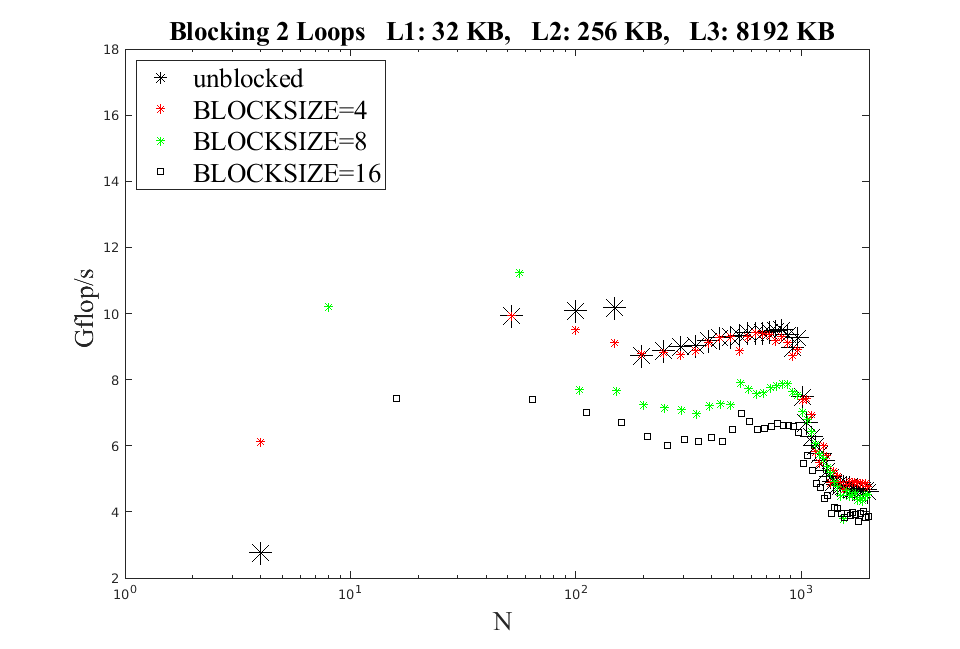
\includegraphics[width=0.8\textwidth]{Fig_3.png}
  \caption{Flop rate versus matrix dimension N for the 'jpi'
           loop ordering and blocking of the two innermost loops,
           for various values of BLOCK\_SIZE.}
  \label{fig3}
\end{figure}

\begin{thebibliography}{99}

\bibitem{dgemm} http://www.netlib.org/lapack/lapack-3.1.1/html/dgemm.f.html

\end{thebibliography}

\end{document}
